\documentclass[10pt,conference]{IEEEtran}

\usepackage[backend=bibtex]{biblatex}
\bibliography{database.bib}
%% \usepackage[fleqn]{amsmath}
\usepackage[margin=1in]{geometry}
\usepackage{amsmath,amsfonts,amsthm,bm}
\usepackage{breqn}
\usepackage{amsmath}
\usepackage{amssymb}
\usepackage{tikz}
\usepackage{algorithm2e}
\usepackage{siunitx}
\usepackage{graphicx}
\usepackage{subcaption}
%% \usepackage{datetime}
\usepackage{multirow}
\usepackage{multicol}
\usepackage{mathrsfs}
\usepackage{fancyhdr}
\usepackage{fancyvrb}
\usepackage{parskip} %turns off paragraph indent
\pagestyle{fancy}

\usetikzlibrary{arrows}

\DeclareMathOperator*{\argmin}{argmin}
\newcommand*{\argminl}{\argmin\limits}

\DeclareMathOperator*{\argmax}{argmax}
\newcommand*{\argmaxl}{\argmax\limits}

\newcommand{\mathleft}{\@fleqntrue\@mathmargin0pt}
\newcommand{\R}{\mathbb{R}}
\newcommand{\Z}{\mathbb{Z}} 
\newcommand{\N}{\mathbb{N}}
\newcommand{\norm}[1]{\|#1\|}
\newcommand{\ppartial}[2]{\frac{\partial #1}{\partial #2}}
\newcommand{\set}[1]{\{#1\}}

\setcounter{MaxMatrixCols}{20}

% remove excess vertical space for align* equations
\setlength{\abovedisplayskip}{0pt}
\setlength{\belowdisplayskip}{0pt}
\setlength{\abovedisplayshortskip}{0pt}
\setlength{\belowdisplayshortskip}{0pt}

\usepackage{multicol}

\begin{document}

\title{Latent Variable Selection with Convex Optimization}
\author{Tina Behrouzi, Yuan Liu}

\markboth{ECE1505 Convex Optimization Project}{}

\maketitle

\section{Abstract}
In this project, we aim to investigate a convex optimization problem for latent variable selection. Its significance include automated determination and interpretation of latent factors which are used in graphical models. Typical construction of graphical models uses some fixed prior or greedy search strategy which are suboptimal and/or non-convergent in general. In our investigation, with access to only observable variables, we aim to decompose the observed relationships into a sparse and a low rank part by formulating as a convex optimization problem, the results of which can fed into graphical model construction which we omit in this paper. We pay special attention to consistency, identifiability and convergence properties of the optimization formulation. Finally, we explore convex optimization solvers for practically solving the problem using real world stock data.
\section{Introduction}
Graph modeling is employed to capture the complicated relationship of variables in a variety of fields, ranging from communication patterns and the stock market to bio information. In graphical model, observed variables are shown as node, and edges indicate connection between them. In practise, lots of time some of the variable are unobserved or latent. Considering these latent variable plays an important role on obtaining the relationship of the data. However, the number and structure of these variables are unknown and difficult to detect. Therefore, determining the structure of latent variables subject to observed ones has been the interest of many studies. The challenge faced when solving this optimization problem on recent data, which usually has high dimensionality and size. 

It is usually considered that latent and observed variables are jointly Gaussian, and the estimation of the covariance matrix between nodes is considered as the representation of the model. Previously, the Expectation-Maximization (EM) algorithm was widely used to learn latent variables of tree-like graphs \cite{xu2017speeding}. However, it has a very slow convergence and poor local optima. Furthermore, the problem can be written as Semidefinite Programming (SDP) format and solved with Interior Point (IP) method in polynomial time \cite{ma2013alternating}. However, it does not consider the sparsity and structure of the problem. Therefore, it is not computationally applicable. 

The method \cite{Chandra_1}, defined the novel solution for finding the structure of the observed variable with respect to the latent variable. The method is based on considering the sparse and low-rank structure for the precision matrix. In section \ref{laten}, we precisely explain the latent variable method \cite{Chandra_1} and its' proof of convergence. In section \ref{comparison},   this method \cite{Chandra_1} is compared based on performance and computational time with other models. The data that we used and the result of the optimization are explained in section \ref{learning}. Finally, the brief conclusion is provided in section \ref{conclusion}.

\section{Latent Variable method} \label{laten}
In this section, first, the main problem is precisely explained. Then, we describe conditions where the algorithm is expected to converge. Finally, the numerical strategy to solve the problem is mentioned.
\subsection*{main problem}
This paper \cite{Chandra_1} considers all observed and latent variable are jointly Gaussian. This is a very common assumption for graphical models' covariance estimation.
Likelihood, assuming normal distribution:
\begin{align*}
  &L(\theta;x) = p_{\theta}(X=x | \theta)\\
  &L(\theta;x) = \frac{1}{(2\pi)^{\frac{D}{2}} (det \Sigma)^{\frac{1}{2}}} exp(-\frac{1}{2}(x-\mu)^T\Sigma^{-1}(x-\mu))\\
  &\theta = (\mu,\Sigma)
\end{align*}
Log likelihood:
\begin{align*}
  l(\theta;x) & = log L(\theta;x)\\
              & = -log((\frac{1}{2 \pi})^{\frac{D}{2}}) - log(det \Sigma)^{\frac{1}{2}}\\
              & - \frac{1}{2}(x-\mu)^T \Sigma^{-1}(x-\mu)
\end{align*}
Optimize over $\theta$:
\begin{align*}
  & \max_{\theta}\ log L(\theta;x)\\
  & \max_{\theta}\ - \frac{1}{2} log(det \Sigma) - \frac{1}{2}(x-\mu)^T \Sigma^{-1}(x-\mu)
\end{align*}
Optimal solution:
\begin{align*}
  & \argmax_{\theta}\ -log(det \Sigma) - (x-\mu)^T \Sigma^{-1}(x-\mu)\\
  &let\ z= x-\mu\ \& \ \Sigma_{s}= zz^T\\
  &let\ K = \Sigma^{-1}\\
  & Therefore, (x-\mu)^T \Sigma^{-1}(x-\mu) = \\
  & tr(z^T \Sigma z) = tr(zz^T \Sigma^{-1}) = tr(\Sigma_{s} K)\\
  & \argmax_{\theta}\ log(det K) - tr(\Sigma_{s} K)\\
\end{align*}
For $K$ positive definite, the above problem can be cast as a convex optimization.\\
 The $X_O \in \mathbb{R}^{p \times 1}$ is the observed variables, and $X_L \in \mathbb{R}^{r \times 1} \:\: r<<p$ indicates the hidden variable. Then we can write $\Sigma_{(O,L)}=[\Sigma_O \; \Sigma_{OL}; \Sigma_{LO} \; \Sigma_L]$ and precision matrix as $K_{(O,L)}=[K_O \; K_{OL}; K_{LO} \; K_L]$. Based on Schur compliment:
 \begin{equation}
     K = \Sigma_O^{-1} = K_O - K_{OL} K_L^{-1} K_{LO}
 \end{equation}
\begin{align*}
  &let\ K=S-L\ The \ Concentration \ matrix \\
  & decomposition \ into \ a \ sparse \ and \ low \ rank \ term.\\
  &let\ S = K_O \ which\ is\ related\ to\ X_O\ condition\ on \ X_L\\
  &let\ L\ = K_{OL} K_L^{-1} K_{LO} \ be \ marginalization\ over\ X_L\\
  &\max_{S,L}\ l(\theta=S-L; \Sigma_{s}) = -\min_{S,L}\ -l(\theta=S-L; \Sigma_{s})\\
\end{align*}
Optimization Formulation:
\begin{align*}
  &\argmin_{S,L} -log det(S-L) + tr(\Sigma_{s}(S-L))\\
  &s.t.\ S-L \succ 0, L \succeq 0\\
\end{align*}
Adding a regularization term (from main paper):
The $l_1$ norm is applied to $S$ to recover sparsity of the matrix, and nuclear norm is used for indicating low-rankness of $L$.
\begin{align}
  \argmin_{S,L}\ & -l(\theta=S-L; \Sigma_{s}) + \lambda(\gamma \|S\|_1 + tr(L))\nonumber\\
  \argmin_{S,L}\ & -log\ det(S-L) + tr(\Sigma_{s}(S-L))\nonumber\\
                 & + \lambda(\gamma \|S\|_1 + tr(L)) \label{mainpro} \\
  s.t.\ & S-L \succ 0, L \succeq 0 \nonumber
\end{align}
Where $\lambda$ is a regularisation term, and $\gamma$ is a trade of between sparsity and rank terms.
\subsection{convergence and optimizer}
\label{converge}
The fisher information, $\mathcal{I}$, is used to provide estimate of certainty, and it is defined as second derivative of the objective function Equ. \ref{mainpro}.
\begin{equation} \nonumber
    \mathcal{I} (K) = K^{-1} \otimes K^{-1} \;\; where \; \otimes is \; tensor\; product
\end{equation}
\begin{itemize}
\item Sparse matrix (observable variables)
\end{itemize}
This is expected not to be densely connected subgraphs, which may otherwise be mistaken for latent variable marginalization. Therefore, a minimum number of zero entries of each row (or matrix degree) should be bounded. To address this point the tangent space and the quantity to measure sparsity are defined as Equ. \ref{sparse}.
\begin{align}
    \Omega(M) = \{ N \in  \mathbb{R}^{p \times p} |  support(N) \subseteq support(M)\}\nonumber\\
    \mu(\Omega(M)) = \underset{N \in \Omega(M), ||N||_{\infty} \leq 1}{max} || N ||_{2} \label{sparse}
\end{align}
Support stands for number of non-zero entries.
\begin{itemize}
\item Low rank matrix (marginalization over latent variables)
\end{itemize}
The $L$ is expected not to be nearly aligned with the coordinate axis in order for increased chance of identifiability. In order to avoid diffusion of latent variables' effect across the observed variables, minimum singular value of matrix should not be too small. Therefore, the tangent space and the quantity to identify that is defined as Equ. \ref{identify}.
\begin{align}
     T(M) = \{ U Y_1^T + Y_2 V^T | Y_1 , Y_2 \in \mathbb{R}^{p \times r}\} \nonumber\\
     \xi(T(M)) = \underset{N \in T(M), ||N||_2 \leq 1}{max} || N ||_{\infty} \label{identify}
\end{align}
Where singular value decomposition of M is $U D V^T$.
The two tangent spaces $T$ and $\Omega$ represent local identifiability around low-rank and sparse matrix. Therefore, if these two spaces have a transverse intersection at the origin (the individual vector can be recovered from the sum), then the consistent estimate for problem \ref{mainpro} can be obtained.

The appropriate measurement for evaluating transversality of tangent spaces is the gain, $P_y A^T \mathcal{I} A P_Y$. Where $\mathcal{I}$ is a fisher information defined above, and $P_Y$ is a projection into $Y$. $A: \mathbb{R}^{p \times p} \times  \mathbb{R}^{p \times p} \to  \mathbb{R}^{p \times p}$ is restricted to cartesian product $Y = \Omega \times T$. The bellow variable are defined to ensure that $\Omega$ and $T$ are identifiable under the map of $\mathcal{I}$. 
\begin{equation*}
    \alpha_{\Omega} = \underset{M \in \Omega, ||M||_{\infty}=1}{min} ||P_{\Omega}\mathcal{I}P_{\Omega}(M)||_{\infty}
\end{equation*}
\begin{equation*}
    \alpha_{T} = \underset{\rho(T, T') \leq \xi(T)/2, M \in T'}{min} \underset{||M||_2 = 1}{min} ||P_{T'}\mathcal{I}P_{T'}(M)||_{2}
\end{equation*}
Where $\rho(T,T')$ measures twisting between projection of $T$ and $T'$. Moreover, $\alpha_T$ and $\alpha_{\Omega}$ represent minimum gain of $\mathcal{I}$ restricted to $\Omega$ and $T'$ (close to $T$), respectively. 

In addition, maximum effect of $\Omega$ and $T'$ in the orthogonal direction of $\Omega^{\perp}$ and ${T'}^{\perp}$, respectively is defined below:
\begin{equation*}
    \delta_{\Omega} = \underset{M \in \Omega, ||M||_{\infty}=1}{max} ||P_{\Omega^\perp}\mathcal{I}P_{\Omega}(M)||_{\infty}
\end{equation*}
\begin{equation*}
    \delta_{T} = \underset{\rho(T, T') \leq \xi(T)/2, M \in T'}{max} \underset{||M||_2 = 1}{max} ||P_{{T'}^{\perp}}\mathcal{I}P_{T'}(M)||_{2}
\end{equation*}
Lastly, the Equ. \ref{bO} and \ref{bT} indicates behaviour of $\mathcal{I}$ in $\ell_2$ and $\ell_{\infty}$ norm. These two quantities combined with $\mu(\Omega)$ and $\xi(T)$ control $\mathcal(I)$ restricted to direct sum of $\Omega \oplus T$.
\begin{equation}
\label{bO}
    \beta_{\Omega} = \underset{M \in \Omega, ||M||_{2}=1}{max} ||\mathcal{I}(M)||_{2}
\end{equation}
\begin{equation}
\label{bT}
    \beta_{T} = \underset{\rho(T, T') \leq \xi(T)/2, M \in T'}{max} \underset{||M||_{\infty} = 1}{max} ||\mathcal{I}(M)||_{\infty}
\end{equation}
\begin{equation}
    \nonumber
    \delta = max(\delta_{\Omega},\delta_T) \ \beta = max(\beta_{\Omega},\beta_T) \ \alpha = min(\alpha_{\Omega},\alpha_T)
\end{equation}
The $\alpha$, $\beta$, and $\delta$ bounds the information $\mathcal{I}$ to $T$ and $\Omega$ spaces.
Main assumption of paper \cite{Chandra_1}:
\begin{equation}
    \exists v \in (0,0.5] \ such \ that \ \frac{\delta}{\alpha} \leq 1-2v
\end{equation}
This assumption is generalization of the Lasso irrepresentability condition \cite{wainwright2009sharp}. 

Let n denote to number of samples ${\{{X_O}^i\}_{i=1}}^n$ of p observed variable. Suppose that $\mu(\Omega) \xi(T) \leq \frac{1}{6}(\frac{v a}{\beta(2-v})^2$ and Equ. \ref{gamma} hold. Also consider $n \gtrsim \frac{p}{{\xi(T)}^4}$, $\lambda \asymp \frac{1}{\xi(T)} \sqrt{\frac{p}{n}}$, $\lambda_min(L*) \gtrsim \frac{1}{\xi(T)^3} \sqrt{\frac{p}{n}}$, and $degree(S*) \gtrsim \frac{1}{\xi(T) \mu(\Omega)} \sqrt{\frac{p}{n}}$. Then the main paper \cite{Chandra_1} proposes that with probability greater than $1-2 e^{-p}$ we can have algebraic correctness \ref{sign} and error bound defined in Equ. \ref{error}.
\begin{equation}
    \label{gamma}
    \gamma \in [\frac{3 \xi(T) \beta(2-v)}{v\alpha},\frac{v\alpha}{2 \mu(\Omega} \beta(2-v)]
\end{equation}
\begin{align}
    \label{sign}
    sign(\hat{S}) = sign(S^*) \ and \ rank(\hat{L}) = rank(L^*) \\ \label{error}
    ||(\hat{S}-\hat{L})^{-1} - {\Sigma_O}^*||_2 \lesssim \frac{1}{\xi(T)} \sqrt{\frac{p}{n}}
\end{align}
Therefore, for choose of $\lambda$ and $\gamma$ in range of $\sqrt{\frac{p}{n}}$ the primal-dual for optimizer can be specified to guarantee optimality. For more detail explanation of convergence proof see \cite{Chandra_1,wang2010solving}.

\textbf{\textit{Optimizer}}: The main paper \cite{Chandra_1} has used general-purpose solvers \cite{wang2010solving}, Newton-CG Primal Proximal Point Algorithm, for optimization in polynomial time. This is a special-purpose solver for logdet problems. 

The Primal Proximal Point algorithm considers that Slater's condition for both primal and dual problems exists. Moreover, both primal and dual are convex. Therefore, the KKT condition is necessary and sufficient for them. This optimizer computes the full eigenvalue decomposition in each iteration. Moreover, this method \cite{Chandra_1} is applicable for high-dimensional problem, where number of latent and observed variable grow simultaneously.

\section{Comparison} \label{comparison}
In this section, the main paper \cite{Chandra_1} is compared with Alternating Thresholded Gradient Descent (AltGD) \cite{xu2017speeding} and Proximal Gradient-based Alternating-Direction Method (PGADM) \cite{ma2013alternating}. The main drawback of the Latent Variable Model (LVM) \cite{Chandra_1} is that R is updated without taking it's low dimensional structure into account. Therefore, the eigenvalues are estimated in each iteration, which causes the high time complexity of the method.
 
The AltGD \cite{xu2017speeding} improves the performance of the LVM for the high-dimensional latent variable setting. For a large value of the dimension r, due to the complexity of eigenvalue decomposition computation of the LVM, the algorithm \cite{Chandra_1} becomes intractable. In AltGD the $L \in \mathbb{R}^{r \times r}$ is breakdown into $-Z Z^T$, where $Z \in \mathbb{R}^{r \times z} \ z \leq r$. Therefore, choosing a small value for the $z$ force the $rank(L) = rank(Z Z^T) \leq rank(Z) \leq z$ to be small. 

As a result, the AlrGD \cite{xu2017speeding} optimization problem is defined as Equ. \ref{AlrGD}. The constraint of Equ. \ref{AlrGD} which is norm zero is not convex. Moreover, if we consider first part of objective ($trace(\Sigma_s (S + Z Z^T))$, the second derivative of that which is $2 \Sigma_s$ is convex if it is Positive Semi-Definite (PSD). One of the method's assumption is that the eigenvalue of the true covariance matrix is finite and bounded bellow with a strictly positive number; therefore, the first term is convex. However, the second term is not convex because although $S+Z Z^T$ is convex(sum of convex and affine function), $-logdet(X)$ is convex and non-increasing; based on composition rule the second term become nonconvex. 

Therefore, in Equ. \ref{AlrGD} both objective and constraint are nonconvex, making the problem nonconvex optimization. Therefore, the AlrGD method applies the gradient descent method with an exact line search on the objective for both $Z$ and $S$ separately considering other variables to be fixed. For employing the constraint on the optimization, the hard-thresholding is applied to $S$ in each iteration, forcing the number of non-zero entries of $S$ to be bounded by $s$.
\begin{align}
    \label{AlrGD}
    \underset{S,Z}{min} <S + Z Z^T, \Sigma_s> - logdet(S + Z Z^T) \\
    subject \ to \ ||S||_0 \leq s \nonumber 
\end{align}
Where $s > 0$ controls sparsity of $S$.
AltGD doesn't consider any restriction for density of matrix $S$ in the problem's objective, because it assumes that for low rank $L^*$ there exists the $\alpha^*$ where $|| L^* ||_{\infty} \leq \frac{\alpha^*}{p}$ and $s^* = ||S^*||_0 \lesssim \frac{p^2}{z {\alpha^*}^2}$.

The statistical error of this technique is $max ( O(\sqrt{\frac{z p}{n}}) , O(\sqrt{\frac{s^* log(d)}{n}}) )$, which is close to the LVM method. However, AltGD processing time is incredibly faster than LVM (Especially for high dimensional $d$) due to not calculating Singular Value Decomposition (SVD) in each iteration. The main time complexity of this algorithm comes from calculating the partial gradient concerning $Z$.

We notice that AltGD \cite{xu2017speeding} is defining the $L$ as $-Z Z^T$, which means it regards L to be Negative Semi-Definite (NSD). The main paper \cite{Chandra_1} considers $L$ to be PSD. Moreover, it \cite{Chandra_1} shows that by replacing constraint $0 \leq L$ with $L \in space(T)$ and changing the objective \ref{mainpro} part of the $trace(L)$ to nuclear norm $||L||_*$, the algorithm will also converge. However, considering $L$ to be completely NSD is in contrast with the structure of the latent variable. We evaluate the performance of algorithm with change of $L = Z Z^T$, and we name it AltGD\_neg. The comparison with the optimum objective of AltGD\_neg, AltGD, and LVM are reported in the next section. 

The PGADM \cite{ma2013alternating} uses classic and gradient-based Altering Direction Method of Multipliers (ADMM) instead of Newton-CG Primal Proximal Point Algorithm (PPA). The PGADM first rewrite the objective \ref{mainpro} as Equ. \ref{PGADM}. This problem is convex, and the objective is separable into three function $f(R)$, $g(S)$, and $h(L)$. However, the constraint is dependent on all variables. In each iteration, variables are updated separately considering proximal mapping of the function considering the other two variables are constant. With good choice of $\alpha$ and $\beta$ this method obtains global convergence. 
\begin{equation}
    min <R,\Sigma_s> - logdet(R) + \alpha ||S||_1 + \beta tr(L) + I(L) \nonumber
\end{equation}
\begin{equation}
subject \ to \ R-S+L = 0 \label{PGADM}
\end{equation}
Where $I(R)$ is zero for $0\leq L$ and else infinity. This method does not compute SVD in each iteration, therefore the algorithm has less time complexity. The ADMM is 5 to 35 times faster than PPA, and the AltGD method is between 30 to 50 times quicker than ADMM.

We should also mention that some new methods consider differential network to be combination of sparse and low-rank matrix, e.g. \cite{na2019estimating}. The differential network is characterized by the contrast of two precision matrices, from two groups of samples distributed according to the latent variable Gaussian graphical model. These methods provide a more robust precision matrix regarding changes in sparsity.
\section{Learning} \label{learning}
For demonstration, we investigate stock price returns of selected interval over time range (see Table \ref{table:stock_experiments}). CVXPY\cite{Diamond} and SDPT3\cite{sdpt3} are used to solve the optimization problem. Due to solvers differences(interior point in SDPT3 and ADMM in CVXPY's SCS backend), they yield results of different accuracy and we find SCS has trouble in making progress and returns warning of inaccurate answers even with increased iteration limits. Hence SDPT3 is chosen as our solver.
\begin{table}[h]
    \centering
    \begin{tabular}{|c|c|}
        \hline
         Tickers \\ \hline
         GOOGL, AMZN, REGN, AMGN, TM, HMC, EA, ATVI\\ \hline
    \end{tabular}
    \caption{Tickers}
    \label{table:ticker_groups}
\end{table}
\begin{table}[h]
    \centering
    \begin{tabular}{|c|c|c|c|}
        \hline
         Return  & & Total\\
         Interval & Time Range & Samples\\ \hline
         weekly & 2005-01-01 to 2018-01-01 & 503\\ \hline
         biweekly & 2005-01-01 to 2018-01-01 & 251\\ \hline
         monthly & 2005-01-01 to 2018-01-01 & 117\\ \hline
    \end{tabular}
    \caption{Stock Experiments}
    \label{table:stock_experiments}
\end{table}
%\begin{figure}[h]
%    \centering
%    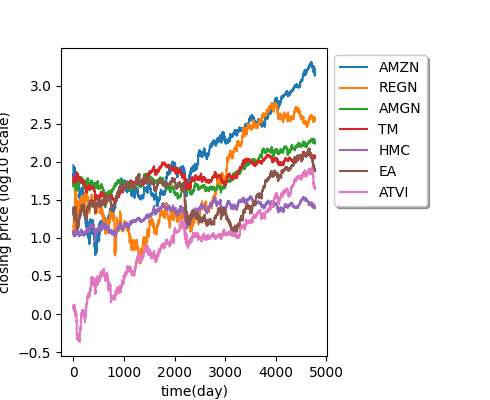
\includegraphics[width=9cm]{imgs/small_2000_2018_1d_2000-01-01_2018-12-31.png}
%    \caption{Raw Data for Selected Stocks from 2000-2018}
%    \label{fig:stock_raw}
%\end{figure}
As noted in \cite{Chandra_2} and seen in previous section, priors of constants related to $\gamma$ and $\lambda$ of the optimization problem Equ. \ref{mainpro} are usually unknown, thus authors perform cross validation on samples to select suitable parameters. We follow this approach by sweeping parameters ($\lambda \in \sqrt{\frac{p}{n}}$, $\gamma \in [0.1,10]$, $n$ is the number of samples, $p$ is the number of observables). We divide total samples $Z$ into training $Z_{train}$ and test $Z_{test}$ respectively in portions of $\frac{4}{5}$ and $\frac{1}{5}$ of the total. We then input them into optimization Equ \ref{mainpro} ($\Sigma_s = \frac{1}{m} Z_{train}Z_{train}^T, Z \in \R^{p \times m}$). $Z_{test}$ is then used along with the output matrices $L$ and $S$ of the optimization problem to give objective value.

Historical stock data are retrieved and returns are calculated as $return_i = (price_{i}-price_{i-1})/price_{i-1}$ for each interval and time range as indicated in Table \ref{table:stock_experiments}. We had considered 2000 to 2018 time range, however it was later found certain companies having missing data and thus shorten the time range to 2005 to 2018. Daily return was considered but not included in our analysis may not reveal as much information due to day trading noise.
\begin{table}[h]
    \centering
    \begin{tabular}{|c|c|c|c|c|}\hline
         Experiment & n & $\sqrt{\frac{p}{n}}$ & $(\lambda,\gamma)_{sel}$ & Objective\\\hline
         weekly & 402 & 0.141 & (0.001, 4.75) & -37.9749 \\ \hline
         biweekly & 200 & 0.200 &(0.0075, 4) & -28.9994 \\ \hline
         monthly  & 93 & 0.293 & (0.01, 5) & -24.0565\\ \hline
    \end{tabular}
    \caption{Solving Parameters: Best objective may not result in most suitable parameters. Here we select suitable parameters based on solved variable characteristics.}
    \label{table:solve_parameters}
\end{table}

\begin{table}[h]
    \centering
    \begin{tabular}{l c c c }
          & S & L & S-L\\
         weekly &  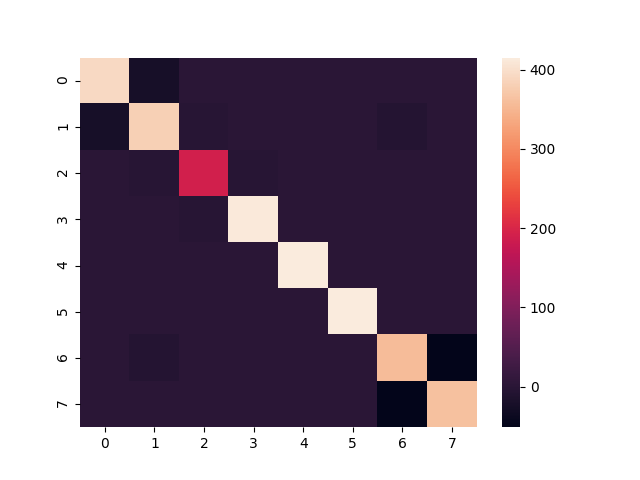
\includegraphics[width=2cm]{imgs/small_weekly_s.png}
         & 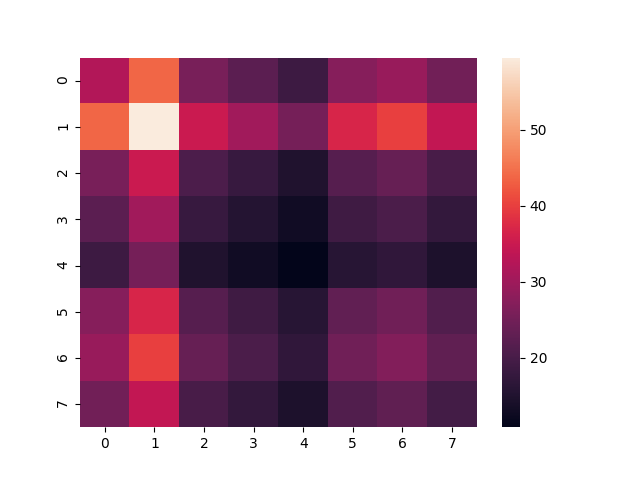
\includegraphics[width=2cm]{imgs/small_weekly_l.png}
         & 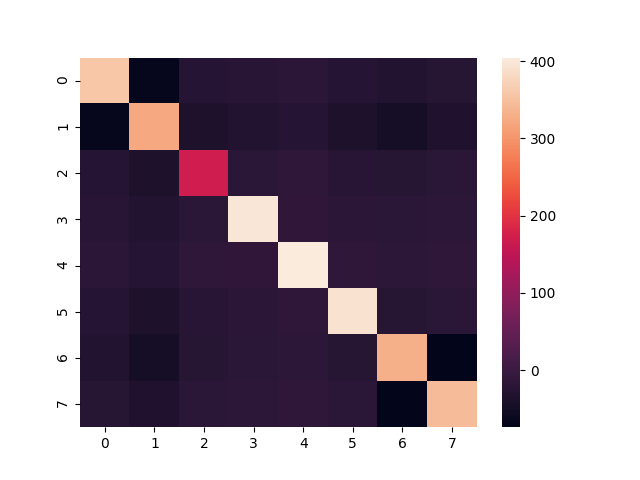
\includegraphics[width=2cm]{imgs/small_weekly_sl.png}\\ 
         biweekly  & 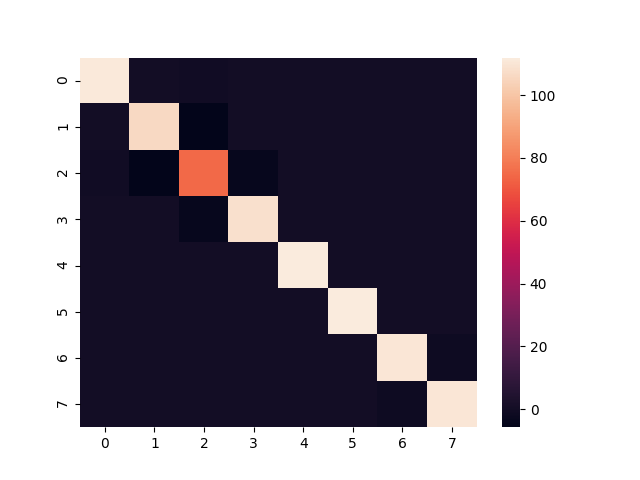
\includegraphics[width=2cm]{imgs/small_biweekly_s.png}
         & 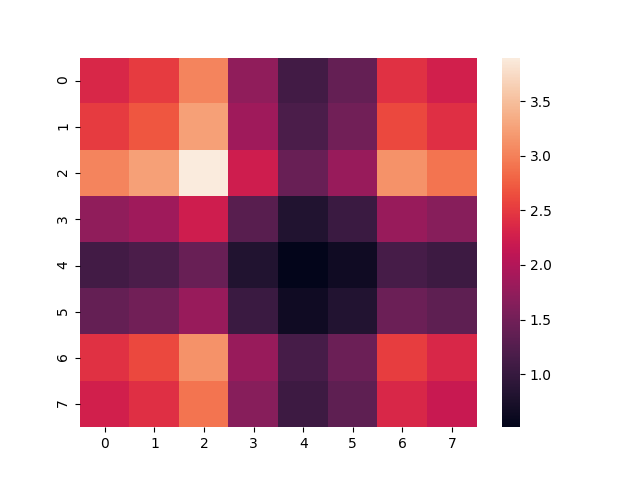
\includegraphics[width=2cm]{imgs/small_biweekly_l.png} 
         & 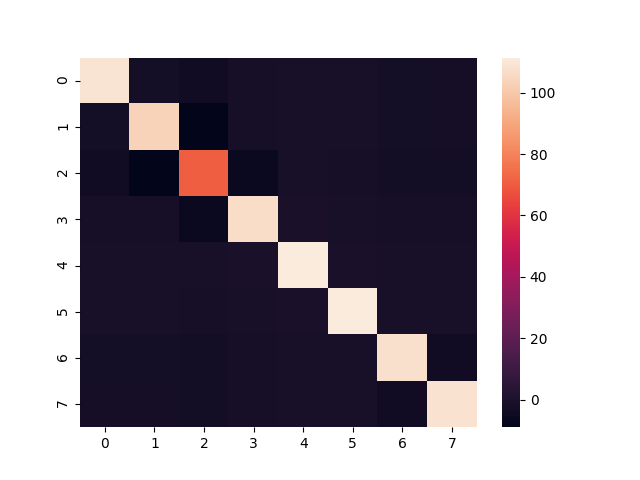
\includegraphics[width=2cm]{imgs/small_biweekly_sl.png}\\ 
         monthly  & 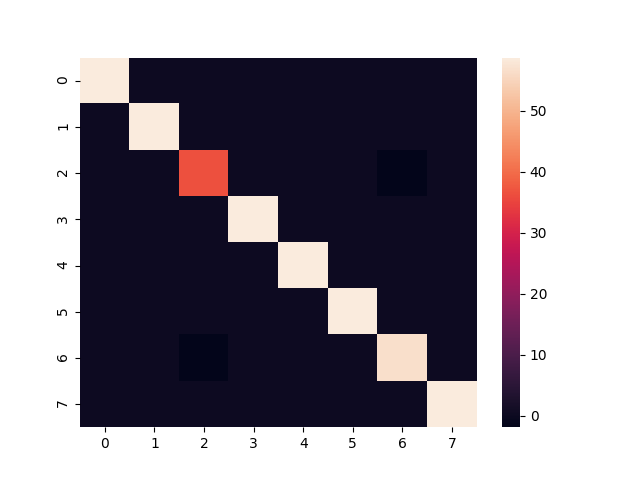
\includegraphics[width=2cm]{imgs/small_monthly_s.png}
        & 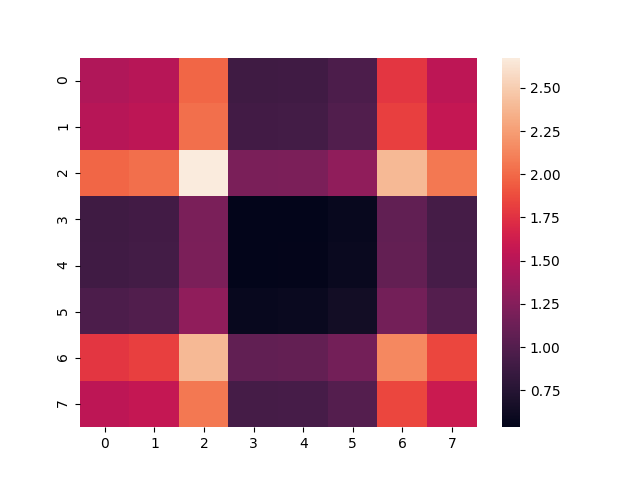
\includegraphics[width=2cm]{imgs/small_monthly_l.png}
        & 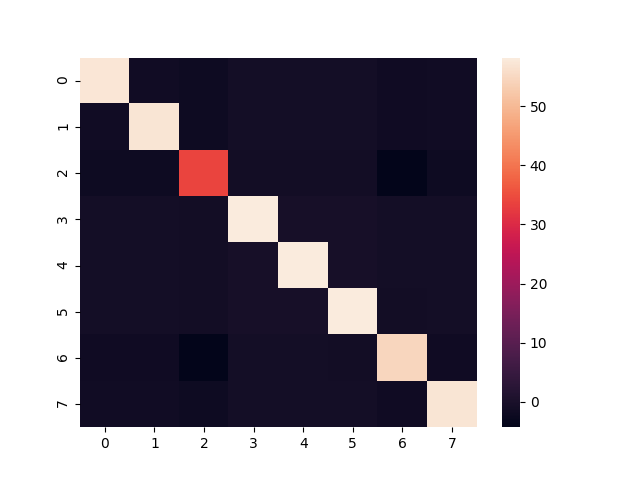
\includegraphics[width=2cm]{imgs/small_monthly_sl.png}\\
    \end{tabular}
    \caption{Solved Variables}
    \label{table:solved_variables}
\end{table}
Parameters are swept so that combined effects of $\lambda$ and $\gamma$ of the sparsity penalization term is near $\sqrt{\frac{p}{n}}$. From examining a typical sweep (see Fig \ref{fig:param_sweep}) and obtained matrices $L, S$, we found that SDPT3 solver returns favourable decrease in objective value at the expense of becoming further away from the ideal regime of $S$ being sparse and $L$ being low rank. 

Using SPDT3, the optimization problem is sensitive to parameters ($\lambda, gamma$). Specifically, parameters were swept at fairly large step sizes at first in order to cover more range and speed up computation, however this tends to miss parameter space in which optimization output has a high dynamic range. We further swept in these regions in order to obtain suitable $S$ and $L$. Parameters resulting in more reasonable $L$ and $S$ are selected in Table \ref{table:solved_variables}. The resulting matrices then describe covariance model of the LVM. Resulting solved $L$ for each experiment is calculated to have 1 non-zero eigenvector and $p-1$ eigenvectors associated with 0 eigenvalue where $L \in \R^{p \times p}$ Since SPDT3 requires hermetian matrix variables for the SDP solver, then rank $L$ is the equal to $p$ minus total number of eigenvectors associated with the zero eigenvalue.
\begin{figure}[h]
    \centering
    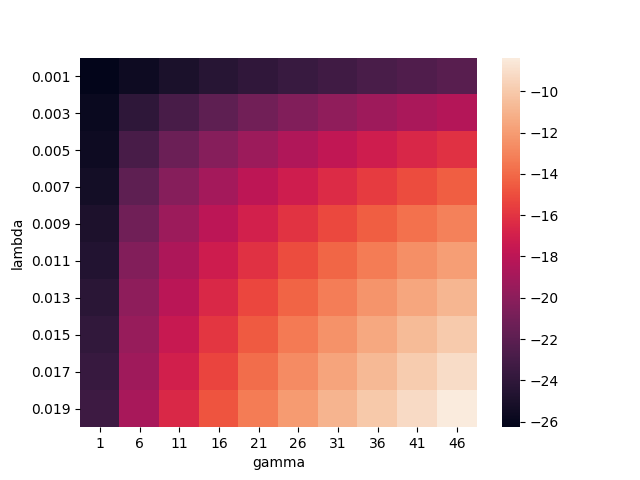
\includegraphics[width=3cm]{imgs/small_sweep_monthly.png}
    \caption{Typical Parameter Sweep $(\lambda,\gamma) \to$ objective of Problem \ref{mainpro}}
    \label{fig:param_sweep}
\end{figure}

\begin{table}[h]
    \centering
    \begin{tabular}{|c|c|c|c|}
        \hline
         Experiment/method & LVM & AltGD & AltGD\_neg \\ \hline
         weekly  & -34.6845 & -34.6997 & -33.4612 \\ \hline
         biweekly & -40.1401 & -40.4255 & -39.8500 \\ \hline
         monthly  & -28.2852 & -24.8420 & -22.0643\\ \hline
    \end{tabular}
    \caption{Comparison of minimum objective derived from AltGD (for z=2) \cite{xu2017speeding}, LVM \cite{Chandra_1}, and AltGD\_neg (Our change to AltGD method)}
    \label{table:comparison}
\end{table}
Based on table \ref{table:comparison}, the minimum objective function of all three methods are very close together. Moreover, considering the $L$ to be PSD has not improved the result of AltGD. The most difference between these methods is simulation time. However, due to small matrices, computation time is around one second for all solvers.
\subsection*{Extensions}
The method can be used for assigning latent interpretation. In \cite{Chandra_2}, latent variables are identified and matched with potential covariates data that are also provided (such as currency exchange rate, GPD index, inflation rate) alongside with observable variables. A set of candidate factor models are tested using specialized matching algorithm.

\section{Conclusion} \label{conclusion}
In conclusion latent model inference and selection is tackled by assuming a graphical model from the exponentially family conditioned on latent variables and formulating it as a logdet convex optimization problem. We investigated the main paper \cite{Chandra_1} and expanded in detail its related and surrounding literature. Conditions for identifiability, convergence were studied in which authors further gave validation using known synthetic data generator of desired properties.
Due to dependency on sensitive parameters, practical implementation typically involve rough estimations of parameter range, as indicated by the main authors and this difficulty is also encountered in our experiments using real world data. Additionally, different optimization methods were explored in experiments where we found varying degrees of satisfaction of the generated solution from CVXPY's SCS, SPDT3, and AltGD. From this observation, it is likely that real world stock data used in our experiment is itself challenging due to lack of externally provided signals which might aid in the inference. 

\section*{References}
\printbibliography[heading=none]

\end {document}